\chapter{Frieze Patterns}

\begin{quote}
Architecture in general is frozen music.

\hfill---Friedrich Wilhelm Joseph von Schelling 
%In this universe, there's only one absolute\dots everything freezes!

%\hfill---Mr.\ Freeze
\end{quote}


\section{Design in a Line}

In design and architecture, a \index{frieze pattern}\textit{frieze},
pronounced ``freeze,'' is a horizontal band that is found near the
ceiling or roof. It is often decorated with a repeating design. Let's
see some examples:
\begin{center}
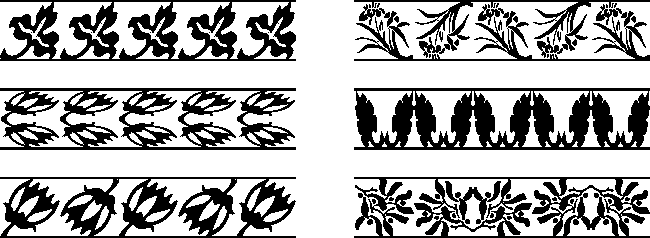
\includegraphics{../graphics/fpfrieze.pdf}
\end{center}
In each case, the pattern above can be thought of as an infinite strip
with the pattern continuing indefinitely.  Frieze patterns often have
symmetry in their structure. While in real-life, the symmetry would
not be perfect, it is useful in mathematics to simplify reality by
replacing the real patterns by idealized designs.  In this chapter, we
will study the symmetry of frieze patterns. At this point we will
refrain from giving a rigorous definition of a \textit{frieze
  pattern}. Instead, this will be a result of our work in this
chapter.


\break

\subsection{Symmetries}

\subsection*{Translations}\index{translation}

Perhaps the most apparent symmetry that frieze patters can exhibit is
symmetry through \textit{horizontal translations}:
\begin{center}

\includegraphics{../graphics/fptrans.pdf}
\end{center}
We will not only insist that a frieze pattern always have
translational symmetry, but we will also insist that such a
translation is \textit{discrete}, meaning that it occurs in distinct
``hops'' of some minimal distance. So, for example, the while the
following patterns have minimal discrete translations, 
\begin{center}

\includegraphics{../graphics/fptransDis.pdf}
\end{center}
this pattern
\begin{center}

\includegraphics{../graphics/fptransNot.pdf}
\end{center}
does not, and hence will not technically be considered a frieze
pattern. To be completely explicit: 
\begin{center}
\textbf{All frieze patterns have symmetry through a minimal discrete
  horizontal translation.}
\end{center}
\begin{dfn}\index{minimal cell}
A \textbf{minimal cell} is the smallest slice of a frieze
pattern that will produce the entire frieze pattern through horizontal
translations.
\end{dfn}

\begin{war}
The minimal cell of a frieze pattern is not unique! Consider
\begin{center}
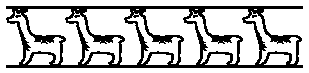
\includegraphics{../graphics/fptransMinEG.pdf}
\end{center}
both
\begin{center}
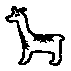
\includegraphics{../graphics/fptransMinEGCell.pdf} \qquad\text{and}\qquad  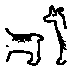
\includegraphics{../graphics/fptransMinEGCell2.pdf}
\end{center}
are minimal cells.
\end{war} 



\subsection*{Horizontal Reflections}\index{horizontal reflection}

Frieze patterns can have symmetry through \textit{horizontal reflections}:
\[

\includegraphics{../graphics/fphoriz.pdf}
\]
Some frieze patterns have symmetry through horizontal reflections, while
others don't.
\begin{ques} 
Can you identify the frieze patterns below with symmetry through
horizontal reflections?
\[
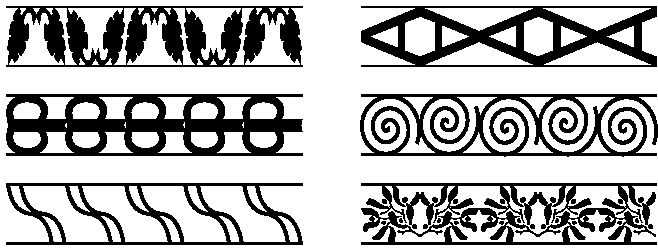
\includegraphics{../graphics/fpfriezeHoriz.pdf}
\]
\end{ques}

\begin{war}
Remember: A horizontal reflection reflects across a vertical line!
\end{war}



\subsection*{Vertical Reflections}\index{vertical reflection}


Frieze patterns can have symmetry through \textit{vertical reflections}:
\[

\includegraphics{../graphics/fpvertical.pdf}
\]

\begin{ques}
Can you identify the frieze patterns below with symmetry through
vertical reflections?
\[
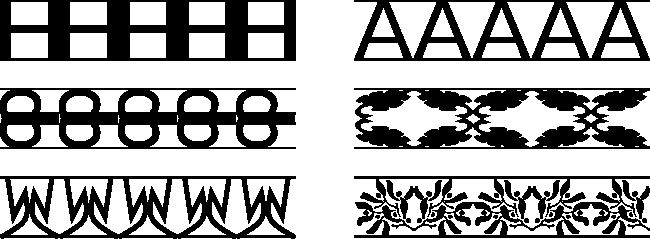
\includegraphics{../graphics/fpfriezeVert-Horiz.pdf}
\]
\end{ques}

\begin{war}
Remember: A vertical reflection reflects across a horizontal
line!
\end{war}




\subsection*{Glide Reflections}\index{glide reflection}

Frieze patterns can have symmetry through \textit{glide reflections}:
\[

\includegraphics{../graphics/fpglide.pdf}
\]

\begin{ques}
Can you identify the frieze patterns below with symmetry through glide
reflections?
\[
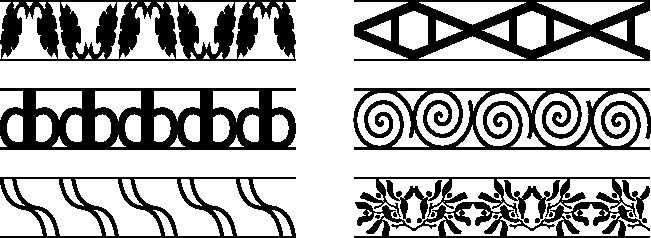
\includegraphics{../graphics/fpfriezeGlide.pdf}
\]
\end{ques}

\begin{ques}
If a frieze pattern has symmetry through translations and vertical
reflections, must it have symmetry through glide reflections?
\end{ques}
\QM




\subsection*{Rotations}\index{rotations}

Finally, frieze patterns can have symmetry through $180^\circ$
rotations.
\[
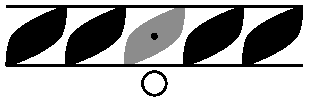
\includegraphics{../graphics/fprot.pdf}
\]

\begin{ques}
Can you identify the frieze patterns below that have symmetry through
$180^\circ$ rotations?
\[
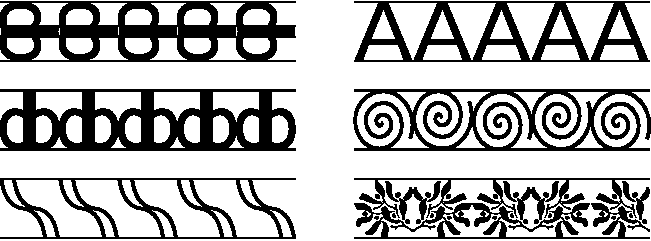
\includegraphics{../graphics/fpfriezeRot.pdf}
\]
\end{ques}

\begin{ques}
Suppose you have a frieze pattern with symmetry through both glide
reflections and $180^\circ$ rotations. Must this pattern also have
symmetry through horizontal reflections?
\end{ques}
\QM


\begin{ques}
Imagine that you have a frieze pattern that has symmetry through
horizontal reflections and $180^\circ$ rotations, but not through
vertical reflections. Could the center of the rotation be on the
vertical line that defines the reflection?
\end{ques}

I think I'll step in and give you a big hint. Consider the following
set of pictures and mysterious symbols:
\[
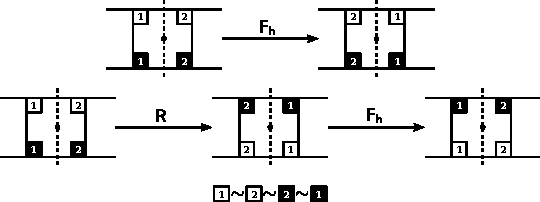
\includegraphics{../graphics/friezeRotRefCent.pdf}
\]
\begin{ques}
Can you explain what these pictures are trying to express?
\end{ques}
\QM


\newpage

\problems
\begin{enumerate}
\item Explain what it means for a frieze pattern to have symmetry
  through horizontal translations. Feel free to draw pictures to help out.
\item Explain what it means for a frieze pattern to have symmetry
  through horizontal reflections. Feel free to draw pictures to help out.
\item Explain what it means for a frieze pattern to have symmetry
  through vertical reflections. Feel free to draw pictures to help out.
\item Explain what it means for a frieze pattern to have symmetry
  through glide reflections. Feel free to draw pictures to help out.
\item Explain what it means for a frieze pattern to have symmetry
  through $180^\circ$ rotations. Feel free to draw pictures to help out.
\item Draw a frieze pattern that exhibits symmetry through horizontal
  translations and identify $3$ different minimal cells.
\item Draw a frieze pattern that exhibits symmetry through horizontal
  translations and glide reflections, but does not have symmetry
  through any other transformation. Be sure to identify a minimal
  cell.
\item Draw a frieze pattern that exhibits symmetry through horizontal
  translations and horizontal reflections, but does not have symmetry
  through any other transformation. Be sure to identify a minimal
  cell.
\item Draw a frieze pattern that exhibits symmetry through horizontal
  translations and $180^\circ$ rotations, but does not have symmetry
  through any other transformation. Be sure to identify a minimal
  cell.
\item Draw a frieze pattern that exhibits symmetry through horizontal
  translations, vertical reflections, and glide reflections, but does
  not have symmetry through any other transformation. Be sure to
  identify a minimal cell.
\item Draw a frieze pattern that exhibits symmetry through horizontal
  translations, horizontal reflections, glide reflections, and
  $180^\circ$ rotations, but does not have symmetry through any other
  transformation. Be sure to identify a minimal cell.
\item Draw a frieze pattern that exhibits symmetry through horizontal
  translations, horizontal reflections, vertical reflections, glide
  reflections, and $180^\circ$ rotations. Be sure to identify a
  minimal cell.
\item Consider the following frieze pattern:
\[
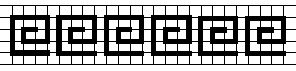
\includegraphics{../graphics/fpGraphEx1.pdf}
\]
Explicitly write down the matrices for the symmetries of this
pattern. Explain your reasoning.
\item Consider the following frieze pattern:
\[
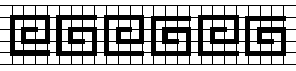
\includegraphics{../graphics/fpGraphEx2.pdf}
\]
Explicitly write down the matrices for the symmetries of this
pattern. Explain your reasoning.
\item Consider the following frieze pattern:
\[
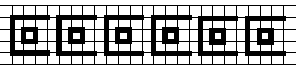
\includegraphics{../graphics/fpGraphEx3.pdf}
\]
Explicitly write down the matrices for the symmetries of this
pattern. Explain your reasoning.
\item Consider the following frieze pattern:
\[
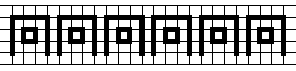
\includegraphics{../graphics/fpGraphEx4.pdf}
\]
Explicitly write down the matrices for the symmetries of this
pattern. Explain your reasoning.
\item Consider the following frieze pattern:
\[
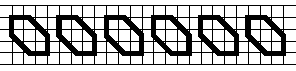
\includegraphics{../graphics/fpGraphEx5.pdf}
\]
Explicitly write down the matrices for the symmetries of this
pattern. Explain your reasoning.
\item Consider the following frieze pattern:
\[
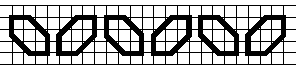
\includegraphics{../graphics/fpGraphEx6.pdf}
\]
Explicitly write down the matrices for the symmetries of this
pattern. Explain your reasoning.
\item Consider the following frieze pattern:
\[
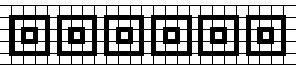
\includegraphics{../graphics/fpGraphEx7.pdf}
\]
Explicitly write down the matrices for the symmetries of this
pattern. Explain your reasoning.
\item Can you exhibit a frieze pattern with 
symmetry through $180^\circ$ rotations but not through glide reflections?
If so, present such a pattern and identify a minimal translation
cell. If not, explain why not.
\item Can you exhibit a frieze pattern with 
symmetry through horizontal reflections but not through glide reflections?
If so, present such a pattern and identify a minimal translation
cell. If not, explain why not.
\item Can you exhibit a frieze pattern with 
symmetry through vertical reflections but not through glide reflections?
If so, present such a pattern and identify a minimal translation
cell. If not, explain why not.
\item Can you exhibit a frieze pattern with 
symmetry through horizontal reflections and $180^\circ$ rotations but not through glide reflections?
If so, present such a pattern and identify a minimal translation
cell. If not, explain why not.


\end{enumerate}

\newpage







\section{Groups---Old and New}

\subsection{Old Friends}


We've already seen some groups. Now we're going to do something
that humans do really well, we're going to give them names.

\subsection*{Groups of Rotations}\index{rotation group}\index{R@$\R_\bullet$}

Consider any regular $n$-gon. We'll let $\R_n$ be the group of
rotations of this $n$-gon. As an example, consider $\R_3$. As we've seen
before, if we let $\mat{R} = \mat{R}_{120}$, then 
\[
\{\mat{I}, \mat{R}, \mat{R}^2\}
\]
forms a group. 

\begin{ques}
What are the elements of $\R_4$? What about $\R_n$?
\end{ques}
\QM

\subsection*{Groups of Reflections}\index{reflection group}\index{F@$\F_\bullet$}

Consider any regular $n$-gon. We'll let $\F_n$ be the group of all
reflections of this $n$-gon. So for a regular $3$-gon, we have
\[
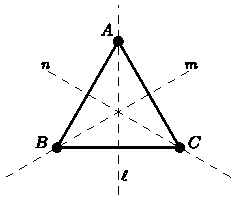
\includegraphics{../graphics/symTriRef.pdf}
\]
Let's write out the group table and see what we get, I've left it
mostly blank. By drawing some pictures, you can do this yourself
(seriously!):
\[
{
\renewcommand{\arraystretch}{1.5}
\begin{array}{| c || c | c | c |c | c | c |}
\hline
\circ & \mat{I} & \mat{F}_\l & \mat{F}_m  & \mat{F}_n & \mat{F}_\l \mat{F}_m &  \mat{F}_\l \mat{F}_n  \\ \hline \hline
\mat{I} &\rule[7mm]{13mm}{0mm} &\rule[7mm]{13mm}{0mm} &\rule[7mm]{13mm}{0mm} &\rule[7mm]{13mm}{0mm} &\rule[7mm]{13mm}{0mm} &  \rule[7mm]{13mm}{0mm}\\ \hline
\mat{F}_\l &\rule[7mm]{13mm}{0mm} & & & & &  \\ \hline
\mat{F}_m &\rule[7mm]{13mm}{0mm} & & & & &  \\ \hline
\mat{F}_n &\rule[7mm]{13mm}{0mm} & & & & &  \\ \hline
\mat{F}_\l\mat{F}_m &\rule[7mm]{13mm}{0mm} & & & & &  \\ \hline
\mat{F}_\l\mat{F}_n &\rule[7mm]{13mm}{0mm} & & & & &  \\ \hline
\end{array}}
\]

Checking with the definition of a group, we see that 
\[
\F_3 = \{ \mat{I}, \mat{F}_\l, \mat{F}_m, \mat{F}_n, \mat{F}_\l\mat{F}_m,\mat{F}_\l\mat{F}_n\}
\]
is indeed a group!

\begin{ques}
How many elements does $\F_n$ have?
\end{ques}
\QM



\subsection*{Symmetry Groups}

We have a special name for the complete symmetry group of a regular
$n$-gon:

\begin{dfn} The \textbf{dihedral group}\index{dihedral
  group}, denoted $\D_n$, is the group of symmetries of a regular
  $n$-gon.
\end{dfn}

\begin{ques}
How many symmetries does a regular $n$-gon have?
\end{ques}
\QM




\subsection{New Friends}


Not only can we make groups from the symmetries of regular $n$-gons,
but we can also make group tables from the symmetries of frieze
patterns. These groups are called \textit{frieze groups}.\index{frieze group}


\subsection*{The Groups $\boldsymbol{\Zt}$ and $\boldsymbol{\Zg}$}

The symmetries of the following frieze pattern form the group $\Zt$:\index{ZT@$\Zt$}
\[
\text{\huge $\Zt$:}\qquad\begin{array}{c}
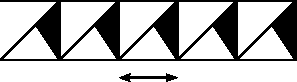
\includegraphics{../graphics/fptransGP.pdf}
\end{array}
\]
This pattern only has symmetry through horizontal translations. Let
$\mat{T}$ represent a translation of the minimal cell to the
right. Then $\mat{T}^{-1}$ is a translation of the minimal cell to the
left. From this we see that
\[
\mat{T}\mat{T}^{-1} = \mat{I}.
\]
Since frieze patterns are thought of as infinite strips, we can apply
a translation successively to itself an infinite number of times---and
each time it will represent a different symmetry of the frieze
pattern. The upshot of this is that a group of symmetries of a frieze
pattern will always have an infinite number of elements. Hence, the
group table will also be infinite. We'll denote this with ``$\cdots$''
in the table so we (meaning you!) can start to write out the partial
group table. Let's do it:
\[
{
\renewcommand{\arraystretch}{1.5}
\begin{array}{| c || c | c | c |c | c | c | c|}
\hline
\circ & \cdots & \mat{T}^{-2} & \mat{T}^{-1}  & \mat{I} & \mat{T} &  \mat{T}^2  & \cdots \\ \hline \hline
\cdots &\cdots & \cdots & \cdots  & \cdots & \cdots &  \cdots &  \cdots\\ \hline
\mat{T}^{-2} & \cdots &\rule[7mm]{13mm}{0mm} &\rule[7mm]{13mm}{0mm} &\rule[7mm]{13mm}{0mm} &\rule[7mm]{13mm}{0mm} &  \rule[7mm]{13mm}{0mm} &  \cdots\\ \hline
\mat{T}^{-1} & \cdots &\rule[7mm]{13mm}{0mm} & & & & & \cdots \\ \hline
\mat{I} & \cdots &\rule[7mm]{13mm}{0mm} & & & & & \cdots \\ \hline
\mat{T} & \cdots &\rule[7mm]{13mm}{0mm} & & & & & \cdots \\ \hline
\mat{T}^2 & \cdots &\rule[7mm]{13mm}{0mm} & & & & & \cdots \\ \hline
\cdots & \cdots & \cdots  &\cdots &\cdots &\cdots &\cdots & \cdots \\ \hline
\end{array}}
\]
Hence:
\[
\Zt = \{\dots, \mat{T}^{-3}, \mat{T}^{-2},\mat{T}^{-1}, \mat{I}, \mat{T},\mat{T}^2,\mat{T}^3, \dots\}
\]


The symmetries of the following frieze pattern form the group $\Zg$:\index{ZG@$\Zg$}
\[
\text{\huge $\Zg$:}\qquad\begin{array}{c}
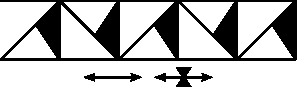
\includegraphics{../graphics/fpglideGP.pdf}
\end{array}
\]
This pattern only has symmetry through horizontal translations and
glide reflections. However, a minimal cell for this frieze pattern is
\[

\includegraphics{../graphics/fpglideMinTransCell.pdf}
\]
We'll let $\mat{T}$ represent the minimal translation of this cell to the
right. On the other hand, a smaller piece of the frieze pattern will
generate the entire pattern through glide reflections.  If we let
$\mat{G}$ represent this glide reflection to the right, we see that
\[
\mat{G}\mat{G}^{-1} = \mat{I} \qquad\text{and}\qquad\mat{G}\mat{G} = \mat{T}.
\]
So we (meaning you!) can start to write out the partial group table:
\[
{
\renewcommand{\arraystretch}{1.5}
\begin{array}{| c || c | c | c |c | c | c | c|}
\hline
\circ & \cdots & \mat{G}^{-2} & \mat{G}^{-1}  & \mat{I} & \mat{G} &  \mat{G}^2  & \cdots \\ \hline \hline
\cdots &\cdots & \cdots & \cdots  & \cdots & \cdots &  \cdots &  \cdots\\ \hline
\mat{G}^{-2} & \cdots &\rule[7mm]{13mm}{0mm} &\rule[7mm]{13mm}{0mm} &\rule[7mm]{13mm}{0mm} &\rule[7mm]{13mm}{0mm} &  \rule[7mm]{13mm}{0mm} &  \cdots\\ \hline
\mat{G}^{-1} & \cdots &\rule[7mm]{13mm}{0mm} & & & & & \cdots \\ \hline
\mat{I} & \cdots &\rule[7mm]{13mm}{0mm} & & & & & \cdots \\ \hline
\mat{G} & \cdots &\rule[7mm]{13mm}{0mm} & & & & & \cdots \\ \hline
\mat{G}^2 & \cdots &\rule[7mm]{13mm}{0mm} & & & & & \cdots \\ \hline
\cdots & \cdots & \cdots  &\cdots &\cdots &\cdots &\cdots & \cdots \\ \hline
\end{array}}
\]
We'll denote this group by:
\[
\Zg = \{\dots, \mat{G}^{-3}, \mat{G}^{-2},\mat{G}^{-1}, \mat{I}, \mat{G},\mat{G}^2,\mat{G}^3, \dots\}
\]


\begin{ques}
What is the connection between the group tables for $\Zt$ and $\Zg$?
\end{ques}
\QM







\subsection*{The Group $\boldsymbol{\Zgf}$}

The symmetries of the following frieze pattern form the group $\Zgf$:\index{ZGF@$\Zgf$}
\[
\text{\huge $\Zgf$:}\qquad\begin{array}{c}

\includegraphics{../graphics/fpverticalGP.pdf}
\end{array}
\]
This pattern only has symmetry through horizontal translations, glide
reflections, and vertical reflections. Let $\mat{T}$ be the horizontal
translation, $\mat{G}$ be the glide reflection, and $\mat{F}$ be the
vertical reflection.

\begin{eg} 
Can you express $\mat{T}$ entirely in terms of $\mat{F}$ and
$\mat{G}$?

Check out these pictures:
\[
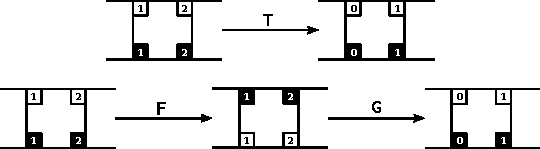
\includegraphics{../graphics/friezeGF-T.pdf}
\]
The first line shows us a translation. The second line shows us
$\mat{G}\mat{F}$. Since they are the same, we've expressed $\mat{T}$
entirely in terms of $\mat{F}$ and $\mat{G}$.
\end{eg}


\begin{ques} Is $\mat{G}\mat{F} = \mat{F}\mat{G}$?
\end{ques}
\QM

\begin{ques}
An arbitrary element of $\Zt$ looks like $\mat{T}^n$. An arbitrary
element of $\Zg$ looks like $\mat{G}^n$. What does an arbitrary element
of $\Zgf$ look like?
\end{ques}
\QM

\begin{eg}
Explain how we know $\Zgf$ is a group.

To do this, we need to check the four parts of the definition of a
group:
\begin{enumerate}
\item Since all of our elements are matrices, and matrix multiplication is associative, we have the needed ``associative operation.''
\item Since $\Zgf$ is the list of all of the symmetries of the frieze
  pattern above, it is necessarily closed under our operation.
\item The identity element $\mat{I}$ is simply the symmetry that
  ``does nothing.''
\item Every element has an inverse, because every transformation can
  be undone.
\end{enumerate}
So $\Zgf$ is a group!
\end{eg}





\subsection*{The Groups $\boldsymbol{\Ztf}$, $\boldsymbol{\Ztr}$, and $\boldsymbol{\Zgr}$}


The symmetries of the following frieze pattern form the group
$\Ztf$:\index{ZTF@$\Ztf$}
\[
\text{\huge $\Ztf$:}\qquad\begin{array}{c}

\includegraphics{../graphics/fphorizGP.pdf}
\end{array}
\]
This pattern only has symmetry through horizontal translations and
horizontal reflections. Let $\mat{T}$ be the horizontal translation
and $\mat{F}$ be the horizontal reflection.

\begin{ques} Is $\mat{T}\mat{F} = \mat{F}\mat{T}$?
\end{ques}
\QM

Once again, we (meaning you!) can start to write out the partial group
table:


\[
{
\renewcommand{\arraystretch}{1.5}
\begin{array}{| c || c | c | c | c | c | c | c | c | c | c|}
\hline
\circ & \cdots & \mat{T}^{-2} & \mat{T}^{-1}\mat{F}  & \mat{T}^{-1} & \mat{I} & \mat{T} &  \mat{F} & \mat{T} \mat{F} & \mat{T}^2  & \cdots \\ \hline \hline
\cdots &\cdots & \cdots & \cdots  & \cdots & \cdots &  \cdots  & \cdots & \cdots &  \cdots &  \cdots\\ \hline
\mat{T}^{-2} & \cdots &\rule[7mm]{13mm}{0mm} &\rule[7mm]{13mm}{0mm} &\rule[7mm]{13mm}{0mm} &\rule[7mm]{13mm}{0mm}  &\rule[7mm]{13mm}{0mm} &\rule[7mm]{13mm}{0mm} &\rule[7mm]{13mm}{0mm} &  \rule[7mm]{13mm}{0mm} &  \cdots\\ \hline
\mat{T}^{-1} \mat{F} & \cdots &\rule[7mm]{13mm}{0mm} & & & & & & & & \cdots \\ \hline
\mat{T}^{-1} & \cdots &\rule[7mm]{13mm}{0mm} & & & & & & & & \cdots \\ \hline
\mat{I} & \cdots &\rule[7mm]{13mm}{0mm} & & & & & & & &\cdots \\ \hline
\mat{T} & \cdots &\rule[7mm]{13mm}{0mm} & & & & & & & & \cdots \\ \hline
\mat{F} & \cdots &\rule[7mm]{13mm}{0mm} & & & & & & & & \cdots \\ \hline
\mat{T} \mat{F} & \cdots &\rule[7mm]{13mm}{0mm} & & & & & & & & \cdots \\ \hline
\mat{T}^2 & \cdots &\rule[7mm]{13mm}{0mm} & & & & & & & &\cdots \\ \hline
\cdots & \cdots & \cdots  &\cdots &\cdots &\cdots &\cdots & \cdots &\cdots &\cdots & \cdots \\ \hline
\end{array}}
\]

\begin{ques}
An arbitrary element of $\Zt$ looks like $\mat{T}^n$. An arbitrary
element of $\Zg$ looks like $\mat{G}^n$. What does an arbitrary element
of $\Ztf$ look like?
\end{ques}
\QM










The symmetries of the following frieze pattern form the group $\Ztr$:\index{ZTR@$\Ztr$}
\[
\text{\huge $\Ztr$:}\qquad\begin{array}{c}

\includegraphics{../graphics/fprotGP.pdf}
\end{array}
\]
This pattern only has symmetry through horizontal translations and
$180^\circ$ rotations. Let $\mat{T}$ be the horizontal translation and
$\mat{R}$ be the $180^\circ$ rotation.

\begin{ques} Is $\mat{T}\mat{R} = \mat{R}\mat{T}$?
\end{ques}
\QM

\begin{ques}
Can you remind us why this is a group?
\end{ques}
\QM

\begin{ques}
An arbitrary element of $\Zt$ looks like $\mat{T}^n$. An arbitrary
element of $\Zg$ looks like $\mat{G}^n$. What does an arbitrary element
of $\Ztr$ look like?
\end{ques}
\QM










The symmetries of the following frieze pattern form the group
$\Zgr$:\index{ZGR@$\Zgr$}
\[
\text{\huge $\Zgr$:}\qquad\begin{array}{c}
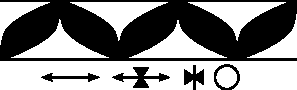
\includegraphics{../graphics/fpzgrGP.pdf}
\end{array}
\]
This pattern only has symmetry through horizontal translations, glide
reflections, horizontal reflections, and $180^\circ$ rotations. Let
$\mat{T}$ be the horizontal translation, $\mat{G}$ be the glide
reflection, $\mat{F}$ be the horizontal reflection, and $\mat{R}$ be
the $180^\circ$ rotation.

\begin{ques} 
Can you express $\mat{T}$ and $\mat{F}$ entirely in terms of $\mat{G}$
and $\mat{R}$?
\end{ques}
\QM
\begin{ques} Is $\mat{G}\mat{R} = \mat{R}\mat{G}$?
\end{ques}
\QM

\begin{ques}
What's the group table of $\Zgr$ going to look like?
\end{ques}
\QM


\begin{ques}
An arbitrary element of $\Zt$ looks like $\mat{T}^n$. An arbitrary
element of $\Zg$ looks like $\mat{G}^n$. What does an arbitrary element
of $\Zgr$ look like?
\end{ques}
\QM









\subsection*{The Group $\boldsymbol{\Ztfr}$}

The symmetries of the following frieze pattern form the group $\Ztfr$:\index{ZTRF@$\Ztfr$}
\[
\text{\huge $\Ztfr$:}\qquad\begin{array}{c}
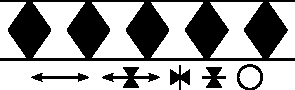
\includegraphics{../graphics/fptfrGP.pdf}
\end{array}
\]
This pattern has symmetry through horizontal translations, glide
reflections, horizontal reflections, vertical reflections and
$180^\circ$ rotations.  Let $\mat{T}$ be the horizontal translation,
$\mat{G}$ be the glide reflection, $\mat{F_h}$ be the horizontal
reflection, $\mat{F_v}$ be the vertical reflection, and $\mat{R}$ be
the $180^\circ$ rotation.


\begin{ques} 
Can you express $\mat{G}$ and $\mat{F_h}$ entirely in terms of $\mat{T}$, $\mat{F_v}$, and $\mat{R}$?
\end{ques}
\QM
\begin{ques} 
Is $\mat{T}\mat{F_v} = \mat{F_v}\mat{T}$? What about $\mat{T}\mat{R} =
\mat{R}\mat{T}$? What about $\mat{F_v}\mat{R} = \mat{R}\mat{F_v}$?
\end{ques}
\QM

Let's start to write out the partial group table:
\[
{
\renewcommand{\arraystretch}{1.5}
\begin{array}{| c || c | c | c | c | c | c | c | c | c | c | c | c|}
\hline
\circ & \cdots & \mat{T}^{-1}\mat{R} & \mat{T}^{-1}\mat{F}  & \mat{T}^{-1} & \mat{I} & \mat{T} &  \mat{F} & \mat{R} & \mat{T}\mat{F} & \mat{T}\mat{R} & \mat{F} \mat{R}  & \cdots \\ \hline \hline
\cdots &\cdots & \cdots & \cdots  & \cdots & \cdots &  \cdots  & \cdots & \cdots &  \cdots &  \cdots &  \cdots &  \cdots\\ \hline
\mat{T}^{-1}\mat{R} & \cdots &\rule[7mm]{8mm}{0mm} &\rule[7mm]{8mm}{0mm} &\rule[7mm]{8mm}{0mm} &\rule[7mm]{8mm}{0mm}  &\rule[7mm]{8mm}{0mm} &\rule[7mm]{8mm}{0mm} &\rule[7mm]{8mm}{0mm} &  \rule[7mm]{8mm}{0mm} &\rule[7mm]{8mm}{0mm} &  \rule[7mm]{8mm}{0mm} &  \cdots\\ \hline
\mat{T}^{-1} \mat{F} & \cdots &\rule[7mm]{8mm}{0mm} & & & & & & & & & & \cdots \\ \hline
\mat{T}^{-1} & \cdots &\rule[7mm]{8mm}{0mm} & & & & & & & & & & \cdots \\ \hline
\mat{I} & \cdots &\rule[7mm]{8mm}{0mm} & & & & & & & & & & \cdots \\ \hline
\mat{T} & \cdots &\rule[7mm]{8mm}{0mm} & & & & & & & & & & \cdots \\ \hline
\mat{F} & \cdots &\rule[7mm]{8mm}{0mm} & & & & & & & & & & \cdots \\ \hline
\mat{R} & \cdots &\rule[7mm]{8mm}{0mm} & & & & & & & & & & \cdots \\ \hline
\mat{T} \mat{F} & \cdots &\rule[7mm]{8mm}{0mm} & & & & & & & & & & \cdots \\ \hline
\mat{T} \mat{R} & \cdots &\rule[7mm]{8mm}{0mm} & & & & & & & & & & \cdots \\ \hline
\mat{F} \mat{R} & \cdots &\rule[7mm]{8mm}{0mm} & & & & & & & & & & \cdots \\ \hline
\cdots & \cdots & \cdots  &\cdots &\cdots &\cdots &\cdots & \cdots &\cdots &\cdots & \cdots &\cdots & \cdots \\ \hline
\end{array}}
\]


\begin{ques}
An arbitrary element of $\Zt$ looks like $\mat{T}^n$. An arbitrary
element of $\Zg$ looks like $\mat{G}^n$. What does an arbitrary element
of $\Ztfr$ look like?
\end{ques}
\QM
\vfill
\break



\paragraph{Some Observations and Thoughts}


Look back at the partial group tables that you have constructed. What
patterns do you notice? Which group tables are fundamentally the same?
Which are different? If we expanded the partial group tables even
more, could you continue to fill them out?



As a gesture of friendship, here is a collection of the frieze groups
along with frieze patterns:
\[
{
\renewcommand{\arraystretch}{4}
\begin{array}{c}
\text{\huge $\Zt$:}\qquad\begin{array}{c}
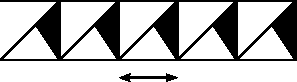
\includegraphics{../graphics/fptransGP.pdf}
\end{array}\\
\text{\huge $\Zg$:}\qquad\begin{array}{c}
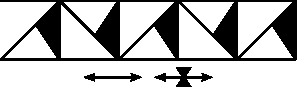
\includegraphics{../graphics/fpglideGP.pdf}
\end{array}\\
\text{\huge $\Zgf$:}\qquad\begin{array}{c}

\includegraphics{../graphics/fpverticalGP.pdf}
\end{array}\\
\text{\huge $\Ztf$:}\qquad\begin{array}{c}

\includegraphics{../graphics/fphorizGP.pdf}
\end{array}\\
\text{\huge $\Ztr$:}\qquad\begin{array}{c}

\includegraphics{../graphics/fprotGP.pdf}
\end{array}\\
\text{\huge $\Zgr$:}\qquad\begin{array}{c}
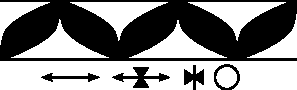
\includegraphics{../graphics/fpzgrGP.pdf}
\end{array}\\
\text{\huge $\Ztfr$:}\qquad\begin{array}{c}
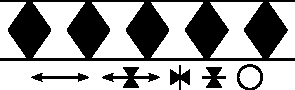
\includegraphics{../graphics/fptfrGP.pdf}
\end{array}
\end{array}
}
\]



\newpage

\problems
\begin{enumerate}
\item State the definition of a group of matrices.
\item Explain what is meant by the symbol $\R_n$. Give an example.
\item If a regular 2-gon is just a line segment, give the group table
  for $\R_2$.
\item Give the group table for $\R_3$.
\item Give the group table for $\R_4$.
\item Give the group table for $\R_5$.
\item How many elements does $\R_n$ have? Explain your reasoning.
\item Explain what is meant by the symbol $\F_n$. Given an example. 
\item If a regular 2-gon is just a line segment, give the group table
  for $\F_2$.
\item Give the group table for $\F_3$.
\item Give the group table for $\F_4$.
\item Give the group table for $\F_5$.
\item How many elements does $\F_n$ have? Explain your reasoning.
\item Explain what is meant by the symbol $\D_n$. Given an example.
\item If a regular 2-gon is just a line segment, give the group table
  for $\D_2$.
\item Give the group table for $\D_3$.
\item Give the group table for $\D_4$.
\item Give the group table for $\D_5$.
\item How many elements does $\D_n$ have? Explain your reasoning.
\item Draw three different frieze patterns whose symmetries are
  described by $\Zt$.
\item Draw three different frieze patterns whose symmetries are
  described by $\Zg$.
\item Draw three different frieze patterns whose symmetries are
  described by $\Zgf$.
\item Draw three different frieze patterns whose symmetries are
  described by $\Ztf$.
\item Draw three different frieze patterns whose symmetries are
  described by $\Ztr$.
\item Draw three different frieze patterns whose symmetries are
  described by $\Zgr$.
\item Draw three different frieze patterns whose symmetries are
  described by $\Ztfr$.
%\item SOMETHING WITH LATTICE DIAGRAMS

\end{enumerate}

\newpage



\section{There Can Be Only Seven}


The title of this section says it all---there are only seven frieze
groups. Believe it or not, we will tackle this monster by solving an
unrelated problem!

\subsection{Pascal's Pizza Shop}

\textit{Pascal's Pizza Shop} makes a variety of pizzas, all which come
with cheese.  However, they do not offer double toppings---no ``double
cheese'' and so on.

\begin{ques}
If he offers two additional toppings, namely basil and garlic.
\begin{enumerate}
\item How many different 1-item pizzas (cheese plus one other
  topping) can he make?  List the possibilities.
\item How many different 2-item pizzas can he make?  List them.
\item How many different 0-item pizzas can he make?
\item In total, how many different pizzas can he make?
\end{enumerate}
\end{ques}
\QM

\begin{ques}
Now suppose he has basil, garlic, and spinach toppings
available.
\begin{enumerate}
\item How many 0-item pizzas can he make?
\item How many 1-item pizzas can he make?
\item How many 2-item pizzas can he make?
\item How many 3-item pizzas can he make?
\item In total, how many different pizzas can he make?
\end{enumerate}
\end{ques}
\QM

\begin{ques}
Complete the following chart by listing and counting the
possibilities, where $n$ is the number of toppings Pascal has
available, and $k$ is the number of toppings used.\\
\[
{\renewcommand{\arraystretch}{2}
\begin{array}{|c||c|c|c|c|c|c||c|}
    \hline
          & k=0 & k=1 & k=2 & k=3 & k=4 & k=5 & \text{Total}\\
    \hline\hline
    n=0 &       &       &       &       &       &    &  \\
    \hline
    n=1 &       &       &       &       &       &    &  \\
    \hline
    n=2 &       &       &       &       &       &    &  \\
    \hline
    n=3 &       &       &       &       &       &    &  \\
    \hline
    n=4 &       &       &       &       &       &    &  \\
    \hline
    n=5 &       &       &       &       &       &    &  \\
    \hline
\end{array}}
\]
\end{ques}
\QM

\begin{ques} 
Often the numbers in the table you filled in above are arranged a bit
differently, as below, where the top ``1" counts the number of
0-topping pizzas that can be made if zero toppings are
available. Complete the first 8 rows of the triangle, which is called
\textit{Pascal's Triangle}.\index{Pascal's Triangle}
\[
\begin{tabular}{c c c c c c c}
      &   &   & 1 &   &   &  \\
      &   & 1 &   & 1 &   &  \\
      & 1 &   & 2 &   & 1 &  \\
    1 &   & 3 &   & 3 &   & 1
\end{tabular}
\vspace{2in}
\]
Do you see some patterns in the triangle?  Describe them and try to
explain why (in terms of pizzas) why they occur.
\end{ques}
\QM



\subsection{Symmetries as Toppings}

We are going to count the various way that a frieze pattern could have
symmetry. Let's list the basic geometric transformations that can
preserve frieze patterns:
\begin{enumerate}
\item Horizontal translations denoted by $\mat{T}$.
\item Horizontal reflections denoted by $\mat{F_h}$.
\item Vertical reflections denoted by $\mat{F_v}$.
\item Glide reflections denoted by $\mat{G}$.
\item Rotations of $180^\circ$ denoted by $\mat{R}$.
\end{enumerate}
Hence, just as we counted pizza's with a number of toppings, we can
count groups of symmetries, where we select groups containing the
transformations above.

To start, not that every frieze pattern has symmetry through horizontal
translations. So we don't need to count that one---this is like saying
that every pizza has cheese on it. Let's list out all possible combinations
of the remaining 4 transformations. To make sure we get them all, we are
going to do this in a very orderly fashion.

\begin{ques} 
How many combinations of symmetries should there be with a single
transformation?  What are they?
\end{ques}
\QM

\begin{ques} 
How many combinations of symmetries should there be with two
transformations?  What are they?
\end{ques}
\QM

\begin{ques} 
How many combinations of symmetries should there be with three
transformations?  What are they?
\end{ques}
\QM

\begin{ques} 
How many combinations of symmetries should there be with four
transformations?  What are they?
\end{ques}
\QM



\subsection{Grouping by Groups}

Now that you have a listing of all possible combinations of the
symmetries of the frieze patterns, let's literally try to group them
by groups---we're going to put the combinations you already found into
the groups we already know. Here are two leading questions to help you
out:


\begin{ques} 
Why must a frieze pattern have symmetry through glide reflections, if
you know it has symmetry through both translations and vertical
reflections?
\end{ques}

I'll take this one, just to show you how it's done. We'll imagine some
sort of generic frieze pattern, and draw the following pictures:
\[
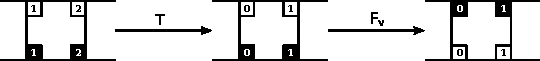
\includegraphics{../graphics/friezeTF-G.pdf}
\]
Hence, from the picture we see that if the frieze pattern has symmetry
through both $\mat{T}$ and $\mat{F_v}$, then it must also have
symmetry through $\mat{G}$.


\begin{ques} 
Why must a frieze pattern have symmetry through $180^\circ$ rotations,
if you know it has symmetry through translations, glide reflections,
and horizontal reflections?
\end{ques}
\QM


\begin{ques} 
Why must a frieze pattern have symmetry through glide reflections, if
you know it has symmetry through translations, horizontal reflections,
and $180^\circ$ rotations?
\end{ques}
\QM

\begin{ques} 
Why must a frieze pattern have symmetry through glide reflections, if
you know it has symmetry through translations, horizontal reflections,
and vertical reflections?
\end{ques}
\QM

\begin{ques} 
Why must a frieze pattern have symmetry through $180^\circ$ rotations, if
you know it has symmetry through translations, horizontal reflections,
and vertical reflections?
\end{ques}
\QM


\begin{ques} 
Why must a frieze pattern have symmetry through vertical reflections,
if you know it has symmetry through translations, horizontal
reflections, and $180^\circ$ rotations?
\end{ques}
\QM




\begin{ques} 
Can you figure out which frieze groups go with which collections of
symmetries you listed above?
\end{ques}
\QM


From this we can finally give a rigorous definition of a frieze pattern
as promised:

\begin{dfn}\index{frieze pattern}
A \textbf{frieze pattern} is a pattern whose symmetries are given by
one of the seven frieze groups.
\end{dfn}




\paragraph{Some Observations and Thoughts}


Now that we have classified all of the frieze groups, let me tell you about
another classification project. Around 1971, a mathematician by the
name of Gorenstein sought to understand \textbf{all} finite
groups. To do this, he proposed that we attempt to classify all of
what are called ``finite simple groups.'' While the definition of a
\textit{simple group} is somewhat beyond the scope of this course, to
put it in SAT terms:
\begin{center}
\textit{simple group} is to \textit{group} \qquad as \qquad \textit{prime number} is to \textit{number}
\end{center}
This goal was eventually finished in 2004---however, the proof of the
classification was enormous. It spanned 15000 pages and required the
work of over 100 mathematicians. Some of the arguments are described
as ``diabolically difficult'' and the proof surely presses to the
limits of human thought.







\newpage

\problems
\begin{enumerate}
\item Suppose you have two toppings, namely basil and garlic.
\begin{enumerate}
\item How many different 0-item pizzas (cheese pizzas) can you make?
\item How many different 1-item pizzas (cheese plus one other topping)
  can you make?  List the possibilities.
\item How many different 2-item pizzas can you make?  List the
  possibilities.
\item In total, how many different pizzas can you  make?
\end{enumerate}
Explain your reasoning.
\item Suppose you have three toppings, namely basil, garlic, and spinach.
\begin{enumerate}
\item How many different 0-item pizzas (cheese pizzas) can you make?
\item How many different 1-item pizzas (cheese plus one other
  topping) can you make?  List the possibilities.
\item How many different 2-item pizzas can you make?  List the
  possibilities.
\item How many different 3-item pizzas can you make?  List the
  possibilities.
\item In total, how many different pizzas can you  make?
\end{enumerate}
Explain your reasoning.
\item Suppose you have four toppings, namely basil, garlic, spinach,
  and tomatoes.
\begin{enumerate}
\item How many different 0-item pizzas (cheese pizzas) can you make?
\item How many different 1-item pizzas (cheese plus one other
  topping) can you make?  List the possibilities.
\item How many different 2-item pizzas can you make?  List the
  possibilities.
\item How many different 3-item pizzas can you make?  List the
  possibilities.
\item How many different 4-item pizzas can you make?  List the
  possibilities.
\item In total, how many different pizzas can you  make?
\end{enumerate}
Explain your reasoning.
\item Write down the first $8$ rows of Pascal's Triangle. Explain what
  each entry means in terms of pizzas and toppings.
\item Describe how to get a new row of Pascal's Triangle from the
  previous row. 
\item Explain in terms of pizzas and toppings why the method described
  in the solution to the previous exercise works.
\item Describe how to find the total number of pizzas one can make
  given a number of toppings.
\item Explain in terms of pizzas and toppings why the method described
  in the solution to the previous exercise works.
\item List the possible symmetries of frieze patterns and give a brief
  explanation of each.
\item How many combinations of symmetries of frieze patterns should
  there be with a single transformation?  What are they? Explain your reasoning.
\item How many combinations of symmetries of frieze patterns should
  there be with two transformations?  What are they? Explain your
  reasoning.
\item How many combinations of symmetries of frieze patterns should
  there be with three transformations?  What are they? Explain your
  reasoning.
\item How many combinations of symmetries of frieze patterns should
  there be with four transformations?  What are they? Explain your
  reasoning.
\item Why must a frieze pattern have symmetry through glide
  reflections, if you know it has symmetry through both translations
  and vertical reflections?
\item Why must a frieze pattern have symmetry through $180^\circ$
  rotations, if you know it has symmetry through translations, glide
  reflections, and horizontal reflections?
\item Why must a frieze pattern have symmetry through glide
  reflections, if you know it has symmetry through translations,
  horizontal reflections, and $180^\circ$ rotations?
\item Why must a frieze pattern have symmetry through glide
  reflections, if you know it has symmetry through translations,
  horizontal reflections, and vertical reflections?
\item Why must a frieze pattern have symmetry through $180^\circ$
  rotations, if you know it has symmetry through translations,
  horizontal reflections, and vertical reflections?
\item Why must a frieze pattern have symmetry through vertical
  reflections, if you know it has symmetry through translations,
  horizontal reflections, and $180^\circ$ rotations?
\item Give three different pictures whose symmetries are described by
  $\R_3$.
\item Give three different pictures whose symmetries are described by
  $\R_4$.
\item Give three different pictures whose symmetries are described by
  $\D_3$.
\item Give three different pictures whose symmetries are described by
  $\D_4$.
\item Consider the simplest frieze group $\Zt$. Can you give a
  pattern that doesn't really resemble a frieze pattern whose
  symmetries are described by this group?
\end{enumerate}
